\section{Rendering}
	
	\begin{frame}[plain, c]
		
	\begin{center}
		\Huge Rendering
	\end{center}
	
	\begin{figure}
				\centering
				\begin{minipage}{.4\paperwidth}
					\centering
					\includegraphics[width=.3\paperwidth]{02_Rendering/img/triangulars.png}
				\end{minipage}%
				\begin{minipage}{.4\paperwidth}
					\centering
					\includegraphics[width=.4\paperwidth]{02_Rendering/img/rendered.png}
				\end{minipage}
		\end{figure}

		
	\end{frame}
	\pdfnote{Whatever}
	\pdfnote{zrdz}
	\pdfnote{zrdz}
	\pdfnote{zrdz}
	\pdfnote{zrdz}
	

		
		% Commands to include a figure:
		%\begin{figure}
		%\includegraphics[width=\textwidth]{your-figure's-file-name}
		%\caption{\label{fig:your-figure}Caption goes here.}
		%\end{figure}
		
	
	\begin{frame}{\Huge{Rendering in der Praxis}}
		
		\begin{figure}
				\centering
				\begin{minipage}{.4\paperwidth}
					\centering
					\includegraphics[width=.4\paperwidth]{02_Rendering/img/journey.jpg}
				\end{minipage}%
				\begin{minipage}{.5\paperwidth}
					\centering
					\includegraphics[width=.4\paperwidth]{02_Rendering/img/cad.jpg}
				\end{minipage}
		\end{figure}
		
		\blfootnote{Bildquellen: \cite{journey, cad}}
		
\end{frame}
	
\begin{frame}{\Huge{Rendering im Film}}
		
		\begin{figure}
				\centering
					\includegraphics[width=.8\paperwidth]{02_Rendering/img/cars.png}
				\centering
		\end{figure}
		
		\begin{itemize}
			\item Komplexe Szenen
			\item Viele Lichtquellen
			\item 24 Bilder pro Sekunde
		\end{itemize}
		
		\blfootnote{Bildquellen: \cite{cars}}
	\end{frame}
	
	\subsection{Licht}
	
\begin{frame}{\Huge{Licht}}
		
		\begin{figure}
				\centering
					\includegraphics[width=.8\paperwidth]{02_Rendering/img/reflexion.png}
				\centering
		\end{figure}
		
		\begin{itemize}
			\item Ideale spekulare Reflexion
			\item Reale spekulare Reflexion
			\item Diffuse Reflexion
		\end{itemize}
		
		\blfootnote{Bildquellen: \cite{reflexion}}
	\end{frame}
	
	\begin{frame}{\colorbox{black!10}{\Huge{Materialien}}}
		
		\begin{figure}
				\centering
					\includegraphics[width=.8\paperwidth]{02_Rendering/img/materials.png}
				\centering
		\end{figure}
		
		\blfootnote{Bildquellen: \cite{realImages}}
	\end{frame}
	
\begin{frame}{\Huge{Lokale Reflexionsmodelle}}
		
		  \begin{tabular}{cl}  
         \begin{tabular}{c}
           \includegraphics[height=3cm, width=3cm]{02_Rendering/img/directLight.png}
           \end{tabular}
           & \begin{tabular}{l}
             \parbox{0.6\linewidth}{%  change the parbox width as appropiate
             \textbf{Bi-Directional Reflection Distribution Function(BRDF)}
             

$$\mathrm{BRDF}=f(\theta_\mathrm{in}, \phi_\mathrm{in}, \theta_\mathrm{ref}, \phi_\mathrm{ref}) = f(\vec{\omega_{i}}, \vec{\omega_{o}})$$
   
    }
         \end{tabular}  \\
\end{tabular}
		
		\blfootnote{Bildquellen: \cite{directLight}}
\end{frame}
	
\begin{frame}{\Huge{Lambertsche Reflexion}}
		
		  \begin{tabular}{cl}  
         \begin{tabular}{c}
           \includegraphics[width=5cm]{02_Rendering/img/lambertian.jpg}
           \end{tabular}
           & \begin{tabular}{l}
             \parbox{0.4\linewidth}{%  change the parbox width as appropiate            

$$I_{D} =\vec{\omega_{i}} \cdot \vec{n}CI_{L}$$


   
    }
         \end{tabular}  \\
\end{tabular}
\end{frame}

\begin{frame}{\Huge{Blinn-Phong BRDF}}
		
		\begin{figure}
				\centering
				\begin{minipage}{.4\paperwidth}
					\centering
					\includegraphics[width=.4\paperwidth]{02_Rendering/img/glossy.jpg}
				\end{minipage}%
				\begin{minipage}{.5\paperwidth}
					\centering
					\includegraphics[width=.4\paperwidth]{02_Rendering/img/h.png}
				\end{minipage}
		\end{figure}
		
    

$$f_{s}(\vec{\omega_{i}}, \vec{\omega_{o}})=\frac{k_{L}}{\pi} + k_{G}\frac{8 + s}{8\pi}z^s$$  $$\mathrm{\quad mit\quad}z=\max(0,\vec{h} \cdot \vec{n})$$
$$\mathrm{\quad mit\quad}\vec{h}=\frac{\vec{\omega_{i}} + \vec{\omega_o}}{2}$$

		\blfootnote{Bildquellen: \cite{h}}  

\end{frame}

\begin{frame}{\Huge{Globale Beleuchtungsmodelle}}
		
		\begin{figure}
				\centering
					\includegraphics[width=.7\paperwidth]{02_Rendering/img/cornellbox.jpg}
				\centering
		\end{figure}

		\blfootnote{Bildquellen: \cite{cornell}}  

\end{frame}

\begin{frame}{\Huge{Die Rendering-Gleichung}}
	
	\begin{center}
		$$L(x, x')=g(x, x') \cdot \lbrack L_e(x,x') + \int_{s} p(x,x',x'')L(x',x'')dx''\rbrack$$
	\end{center}
	
	\begin{itemize}
		\item Analytisch nicht berechenbar
		\item Ann�herung durch Raytracer, Radiosity, etc.
	\end{itemize}
	
\end{frame}

\subsection{Rendering-Techniken}
\begin{frame}{\Huge{Rendering-Techniken}}
	
	\begin{itemize}
		\item Ann�herung an Rendering-Gleichung
		\item Modellkomplexit�t
		\item Model Diversit�t
		\item Komplexes Shading
		\item Geschwindigkeit
		\item Bildqualit�t
		\item Flexibilit�t
	\end{itemize}
	
\end{frame}

\subsubsection{Reyes-Bild-Rendering-Architektur}
\begin{frame}{\Huge{REYES}}
	
	\begin{block}{Problem}
		Komplexe Szenen sind zu gro� um sie komplett im Hauptspeicher zu halten.
	\end{block}
	
	\vskip 1cm
	
	\begin{block}{L�sung}
		Prinzip der geometrischen Lokalit�t
	\end{block}
\end{frame}
\pdfnote{Render Everything you ever saw }

\begin{frame}{\Huge{Maps}}
		\begin{figure}
			\centering
			\begin{minipage}{.4\paperwidth}
				\centering
				\includegraphics[width=.4\paperwidth]{02_Rendering/img/texture.png}
			\end{minipage}%
			\begin{minipage}{.4\paperwidth}
				\centering
				\includegraphics[width=.4\paperwidth]{02_Rendering/img/textured.png}
			\end{minipage}
		\end{figure}
		\begin{figure}
			\begin{minipage}{.4\paperwidth}
				\centering
				\includegraphics[width=.4\paperwidth]{02_Rendering/img/environment.png}
			\end{minipage}
			\begin{minipage}{.4\paperwidth}
				\centering
				\includegraphics[width=.4\paperwidth]{02_Rendering/img/environmented.png}
			\end{minipage}
		\end{figure}
		\blfootnote{Bildquellen: \cite{maps}} 

\end{frame}

\begin{frame}{\Huge{Algorithmus}}

\begin{tabular}{cl}  
	\begin{tabular}{c}
		\includegraphics[width=4.5cm]{02_Rendering/img/reyesalgo.png}
	\end{tabular}
	& \begin{tabular}{l}
		\parbox{0.4\linewidth}{%  change the parbox width as appropiate            
			
		\begin{itemize}
			\item bounding
			\item dicing
			\item splitting
		\end{itemize}
			
		}
	\end{tabular}  \\
\end{tabular}
\blfootnote{Bildquellen: \cite{REYES}} 
\end{frame}

\begin{frame}{\Huge{Algorithmus}}
		\begin{figure}
			\centering
			\begin{minipage}{.4\paperwidth}
				\centering
				\includegraphics[width=.4\paperwidth]{02_Rendering/img/reyesvisible.png}
			\end{minipage}%
			\begin{minipage}{.5\paperwidth}
				\centering
				\includegraphics[width=.4\paperwidth]{02_Rendering/img/sphere.png}
			\end{minipage}
		\end{figure}

	\blfootnote{Bildquellen: \cite{REYES}} 
\end{frame}

\begin{frame}{\Huge{Beispiele}}
	\begin{figure}
		\centering
		\begin{minipage}{.4\paperwidth}
			\centering
			\includegraphics[width=.4\paperwidth]{02_Rendering/img/lamp.png}
		\end{minipage}%
		\begin{minipage}{.5\paperwidth}
			\centering
			\includegraphics[width=.4\paperwidth]{02_Rendering/img/monsterag.png}
		\end{minipage}
	\end{figure}
\blfootnote{Bildquellen: \cite{REYES, monster}} 
\end{frame}

\subsubsection{Raytracing}

\begin{frame}{\Huge{Raytracing}}

	\begin{figure}
		\centering
		\includegraphics[width=.8\paperwidth]{02_Rendering/img/BallsRender.png}
		\centering
	\end{figure}
	\blfootnote{Bildquellen: \cite{rayTracingBalls}} 
\end{frame}

\begin{frame}{\Huge{Reflexionen}}
	\begin{figure}
		\centering
		\begin{minipage}{.4\paperwidth}
			\centering	
			\includegraphics[width=.3\paperwidth]{02_Rendering/img/map.png}
		\end{minipage}%
		\begin{minipage}{.5\paperwidth}
			\centering
			\includegraphics[width=.3\paperwidth]{02_Rendering/img/traced.png}
		\end{minipage}
	\end{figure}
	
		\begin{block}{Vorteile}
			\begin{itemize}
				\item Realistische Reflexionen
				\item Abbildung beliebig vieler Lichtquellen
				\item Spiegelungen spekularer Objekte ineinander
			\end{itemize}
			
		\end{block}
	
	\blfootnote{Bildquellen: \cite{cars}} 
\end{frame}

\begin{frame}{\Huge{Raytracer Algorithmus}}
	

	\begin{figure}

		\begin{minipage}{.5\paperwidth}

			\includegraphics[width=.4\paperwidth]{02_Rendering/img/rayTracing.png}
		\end{minipage}%
		\begin{minipage}{.5\paperwidth}

			\includegraphics[width=.4\paperwidth]{02_Rendering/img/rayTracing2.png}
		\end{minipage}
	\end{figure}
	
	\begin{block}{Performance}
		\begin{itemize}
			\item Schnittpunkttest muss f�r Schatten und Objektberechnung durchgef�hrt werden
			\item Gesamte Szene muss im Hauptspeicher liegen
		\end{itemize}

	\end{block}

	\blfootnote{Bildquellen: \cite{rayTracing}} 
\end{frame}

\begin{frame}{\Huge{H�llk�rper}}
	
	
 \begin{tabular}{cl}  
 	\begin{tabular}{c}
 		\includegraphics[width=4cm]{02_Rendering/img/rabbit.jpg}
 	\end{tabular}
 	& \begin{tabular}{l}
 		\parbox{0.6\linewidth}{%  change the parbox width as appropiate            
 			
 		\begin{itemize}
 			\item H�llk�rper zeichnen leichte Schnittpunktberechnung aus
 			\item H�llk�rper k�nnen Gruppen von Objekten umgeben
 		\end{itemize}
 			
 			
 			
 		}
 	\end{tabular}  \\
 \end{tabular}
	
	\blfootnote{Bildquellen: \cite{rabbit}} 
\end{frame}

\begin{frame}{\Huge{Strahlenb�ndel}}
	
	
	\begin{tabular}{cl}  
		\begin{tabular}{c}
			\includegraphics[width=4.5cm]{02_Rendering/img/raydiffer.jpg}
		\end{tabular}
		& \begin{tabular}{l}
			\parbox{0.6\linewidth}{%  change the parbox width as appropiate            
				
				\begin{itemize}
					\item Nachbarstrahlen beschreiten anfangs einen �hnlichen Weg
					\item Strahlenb�ndelschnittpunkte erzeugen neue Strahlenb�ndel
				\end{itemize}
				
				
				
			}
		\end{tabular}  \\
	\end{tabular}
	
	\blfootnote{Bildquellen: \cite{raydiff}} 
\end{frame}


\begin{frame}{\Huge{Beispiele}}
	
	
	\begin{figure}
		\centering
		\begin{minipage}{.5\paperwidth}
			
			\includegraphics[width=.4\paperwidth]{02_Rendering/img/raytracerCars.png}
		\end{minipage}%
		\begin{minipage}{.5\paperwidth}
			\includegraphics[width=.35\paperwidth]{02_Rendering/img/firstSzene.jpg}
		\end{minipage}
	\end{figure}
	
	\blfootnote{Bildquellen: \cite{cars, firstSzene}} 
\end{frame}

\subsection{Einf�gen eines synthetischen Models in eine reale Szene}
\begin{frame}{\Huge{Synthetisches Model + reale Szene}}
	
	
	\begin{figure}
		\centering
		\includegraphics[width=.7\paperwidth]{02_Rendering/img/gollum.jpg}
	\end{figure}
	
	\blfootnote{Bildquellen: \cite{gollum}} 
\end{frame}

\begin{frame}{\Huge{Szenen Teile}}
	
	
	\begin{tabular}{cl}  
		\begin{tabular}{c}
			\includegraphics[width=4.5cm]{02_Rendering/img/scenes.png}
		\end{tabular}
		& \begin{tabular}{l}
			\parbox{0.6\linewidth}{%  change the parbox width as appropiate            
				
				\begin{itemize}
					\item Distanzszene
					\item Lokale Szene
					\item Synthetisches Objekt
				\end{itemize}
			}
		\end{tabular}  \\
	\end{tabular}
	
	\blfootnote{Bildquellen: \cite{realImages}} 
\end{frame}

\begin{frame}{\Huge{Lichtbasiertes Model der Distanzszene}}
	
	\begin{itemize}
		\item Unabh�ngig von anderen Teilen der Szene
		\item Hauptverantwortlich f�r Beleuchtung der Szene
		\item Ben�tigt genaue Informationen �ber die Lichtintensit�t an jedem Pixel
		\item Intensit�t wird in High Dynamic Ranger Images gespeichert
	\end{itemize}

\end{frame}

\begin{frame}{\Huge{Materialbasiertes Model der lokalen Szene}}
	
	\begin{figure}
		\centering
		\begin{minipage}{.5\paperwidth}
			
			\includegraphics[width=.4\paperwidth]{02_Rendering/img/background.png}
		\end{minipage}%
		\begin{minipage}{.5\paperwidth}
			\includegraphics[width=.35\paperwidth]{02_Rendering/img/localSzeneOnly.png}
		\end{minipage}
	\end{figure}
	
	\begin{itemize}
		\item Empf�ngt Schatten und Reflexion von synthetischen Model
		\item Kann Licht auf synthetisches Model werfen und es verdecken
		\item Muss sowohl Beleuchtungs- als auch Materialeigenschaften vorweisen(BRDFS)
	\end{itemize}

	\blfootnote{Bildquellen: \cite{realImages}} 
	
\end{frame}

\begin{frame}{\Huge{Synthetisches Model}}
	
	\begin{figure}
		\centering
		\begin{minipage}{.5\paperwidth}
			
			\includegraphics[width=.4\paperwidth]{02_Rendering/img/model1.png}
		\end{minipage}%
		\begin{minipage}{.5\paperwidth}
			\includegraphics[width=.35\paperwidth]{02_Rendering/img/model2.png}
		\end{minipage}
	\end{figure}
	
\end{frame}

\begin{frame}{\Huge{Sonderf�lle}}
	
	\begin{itemize}
		\item Konzentriertes Licht bestrahlt das synthetische Model und dieses verursacht starke Schatten
		\item Konzentriertes Licht bestrahlt ein spiegelndes, synthetische Model und dieses wirft Licht in die Szene
		\item Spekulare Oberfl�chen der Distanzszene k�nnen vom Model beeinflusst werden
		\item Das synthetische Model strahlt Licht aus
	\end{itemize}
	
\end{frame}

\subsubsection{Beleuchtung}

\begin{frame}{\Huge{Beleuchtung}}
	
		\begin{tabular}{cl}  
			\begin{tabular}{c}
				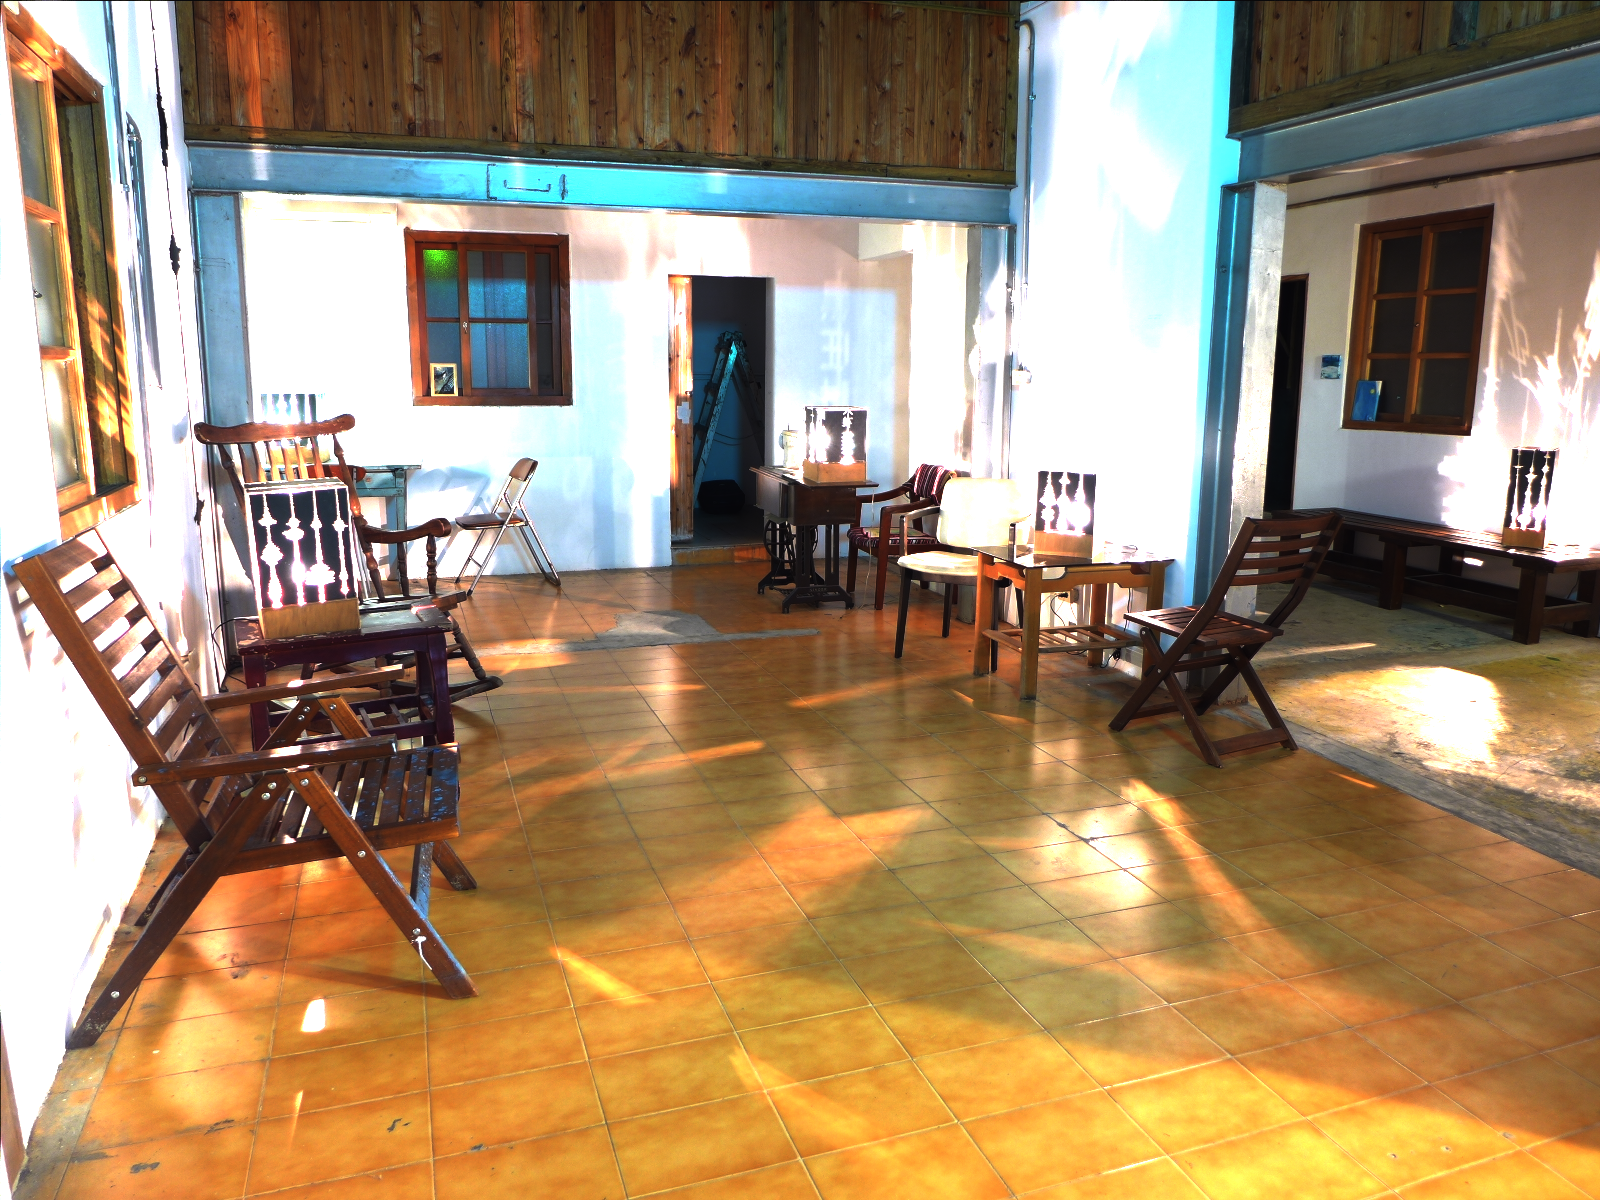
\includegraphics[width=4.5cm]{02_Rendering/img/room.png}
			\end{tabular}
			& \begin{tabular}{l}
				\parbox{0.6\linewidth}{%  change the parbox width as appropiate            
					
					\begin{itemize}
						\item Kann manuell geschehen
						\item Intensit�ten m�ssen gesch�tzt werden
						\item Globale Beleuchtung muss modelliert werden
					\end{itemize}
				}
			\end{tabular}  \\
		\end{tabular}
\end{frame}

\begin{frame}{\Huge{Automatisierte Beleuchtung}}
	
	\begin{figure}
		\centering
		\begin{minipage}{.2\paperwidth}
			\includegraphics[width=.2\paperwidth]{02_Rendering/img/prob1.jpg}
		\end{minipage}%
		\begin{minipage}{.2\paperwidth}
			\includegraphics[width=.2\paperwidth]{02_Rendering/img/prob2.jpg}
		\end{minipage}
		\begin{minipage}{.2\paperwidth}
			\includegraphics[width=.2\paperwidth]{02_Rendering/img/propfull.jpg}
		\end{minipage}
	\end{figure}
	
	\begin{itemize}
		\item Erstellen mehrerer HDRI einer Spiegelkugel
		\item Verschmelzen der HDRIs zum erstellen einer Lichtsonde
	\end{itemize}
	
\end{frame}

\begin{frame}{\Huge{Lichtbasiertes Model erstellen }}
	
		\begin{tabular}{cl}  
			\begin{tabular}{c}
				\includegraphics[width=.4\paperwidth]{02_Rendering/img/algo3.png}
				\includegraphics[width=.4\paperwidth]{02_Rendering/img/distantszene.png}
			\end{tabular}
			& \begin{tabular}{l}
				\parbox{0.6\linewidth}{%  change the parbox width as appropiate            
					
					\begin{itemize}
						\item Kann manuell geschehen
						\item Intensit�ten m�ssen gesch�tzt werden
						\item Globale Beleuchtung muss modelliert werden
					\end{itemize}
				}
			\end{tabular}  \\
		\end{tabular}
	
	\begin{itemize}
		\item Strahlen bis Schnittpunkt mit Box verfolgen
	\end{itemize}
	
		\blfootnote{Bildquellen: \cite{realImages}} 
\end{frame}

\begin{frame}{\Huge{Ergebnis}}
	
	\begin{figure}
		\centering
		\includegraphics[width=.4\paperwidth]{02_Rendering/img/algo4.png}
	\end{figure}
	
	\begin{itemize}
		\item Raytracing zum rendern der Szene
		\item Strahlen vom Model �ber die lokale Szene bis in die Distanzszene verfolgen
	\end{itemize}
		\blfootnote{Bildquellen: \cite{realImages}} 
\end{frame}

\begin{frame}{\Huge{Einf�gen des synthetischen Models}}
		\begin{figure}
			\centering
			\begin{minipage}{.4\paperwidth}
				\centering
				\includegraphics[width=.4\paperwidth]{02_Rendering/img/background.png}
			\end{minipage}%
			\begin{minipage}{.4\paperwidth}
				\centering
				\includegraphics[width=.4\paperwidth]{02_Rendering/img/calibration.png}
			\end{minipage}
		\end{figure}
		\begin{figure}
			\begin{minipage}{.4\paperwidth}
				\centering
				\includegraphics[width=.4\paperwidth]{02_Rendering/img/localszene.png}
			\end{minipage}
			\begin{minipage}{.4\paperwidth}
				\centering
				\includegraphics[width=.4\paperwidth]{02_Rendering/img/final.png}
			\end{minipage}
		\end{figure}
		\blfootnote{Bildquellen: \cite{realImages}} 
\end{frame}


\begin{frame}{\Huge{Fazit}}
	
		\begin{block}{Vorteile}
			\begin{itemize}
				\item Geometrie- und Materialeigenschaften f�r lokale Szene m�ssen nur einmal bestimmt werden
				\item Lichtbasiertes Model der Distanzszene muss nur einmal bestimmt werden
				\item Beleuchtung wirkt korrekt auf synthetische Objekte ein
			\end{itemize}
		\end{block}
		
		
		\begin{block}{Nachteile}
			\begin{itemize}
				\item BRDFs f�r lokale Szene k�nnen nur gesch�tzt werden
				\item Kamera muss kalibriert werden
			\end{itemize}
		\end{block}
\end{frame}

